\documentclass[11pt, oneside]{article}   	% use "amsart" instead of "article" for AMSLaTeX format
\usepackage{geometry}                		% See geometry.pdf to learn the layout options. There are lots.
\geometry{letterpaper}                   		% ... or a4paper or a5paper or ... 
%\geometry{landscape}                		% Activate for rotated page geometry
%\usepackage[parfill]{parskip}    		% Activate to begin paragraphs with an empty line rather than an indent
\usepackage{graphicx}				% Use pdf, png, jpg, or eps§ with pdflatex; use eps in DVI mode
								% TeX will automatically convert eps --> pdf in pdflatex		
\usepackage{amssymb,amsmath}
\usepackage{amsthm}
\usepackage{float}
\usepackage{bm}


\usepackage{listings}
\usepackage[utf8]{inputenc}
\newcommand{\Var}{\operatorname{Var}}
\newcommand{\E}{\operatorname{E}}
\newcommand{\Cov}{\operatorname{Cov}}
% Default fixed font does not support bold face
\DeclareFixedFont{\ttb}{T1}{txtt}{bx}{n}{12} % for bold
\DeclareFixedFont{\ttm}{T1}{txtt}{m}{n}{12}  % for normal

\lstset{language=R,
    basicstyle=\small\ttfamily,
    stringstyle=\color{DarkGreen},
    otherkeywords={0,1,2,3,4,5,6,7,8,9},
    morekeywords={TRUE,FALSE},
    deletekeywords={data,frame,length,as,character},
    keywordstyle=\color{blue},
    commentstyle=\color{DarkGreen},
     %frame=single, % adds a frame around the code
     backgroundcolor=\color{lightgray},
}
\usepackage[svgnames]{xcolor}
\title{STAT211 Mandatory Homework 4}
\author{Yapi Donatien Achou}
%\date{}							% Activate to display a given date or no date

\begin{document}

\maketitle
\tableofcontents
\newpage
 
\section{Problem 4.1}
Consider an ARMA(p,q) model 
\begin{equation}\label{eq:arma}
X_{t}-\sum_{k=1}^{p}\phi_{k}X_{t-k} = Z_{t}+\sum_{k=1}^{p}\theta_{k}Z_{t-k}
\end{equation}
\subsection{Part a: Invertibility}
An ARMA(p,q) process $\{  X_{t}\}$ is invertible if there exist constant $\{  \pi_{j}\}$ such that 
\begin{equation}
\sum_{j=0}^{\infty}|\pi_{j}| \le \infty
\end{equation}
and 
\begin{equation}\label{eq:z}
Z_{t} = \sum_{j=0}^{\infty}\pi_{j}X_{t-j} \quad \text{for all t}.
\end{equation}
In other word $\{  X_{t}\}$ is invertible if $Z_{t}$ can be written as a linear combination of $X_{t-j}$, $j = 0,1, \dots, \infty$, \cite{petter}.

\begin{flushleft}
Invertibility is equivalent to 
\begin{equation}\label{eq:theta}
\theta(z) = 1+ \theta_{1}z+ \cdots + \theta_{q}z^{q}\neq 0 \quad \text{for all} \quad |z| \leq 1
\end{equation}
where $\theta(z)$ is the moving average polynomial.
\end{flushleft}

\begin{flushleft}
The process $X_{t}$ is invertible if and only if the zeros of the moving average polynomial $\theta(z)$ lie outside the unit circle.
%Now let prove that if a process is invertible then $Z_{t}$ is expressible in terms of $X_{s}$, $s\leq t$, given that $|\theta| < 1$.
\end{flushleft}

\subsection{Part b: Linear filter ${\pi_{j}}$}
The sequence $\{\pi_{j}\}$ in (\ref{eq:z}) is determined by the relation
\begin{equation}\label{eq:main}
(1+\theta_{1}z +\theta_{2}z^{2} + \cdots + \theta_{q}z^{q})(\pi_{0} + \pi_{1}z + \cdots) = (1-\phi_{1}z-\phi_{2}z^{2}-\cdots-\phi_{p}z^{q}).
\end{equation}
Multiplying the left hand side together gives 
\begin{equation}
\begin{aligned}
(1+\theta_{1}z +\theta_{2}z^{2} + \cdots + \theta_{q}z^{q})(\pi_{0} + \pi_{1}z + \cdots)&=\pi_{0}+\pi_{1}z+\pi_{2}z^{2}+\cdots +\theta_{1}\pi_{0}z+\theta_{1}\pi_{1}z^{2}+\cdots+\theta_{2}\pi_{0}z^{2}\\
&=\pi_{0}+(\pi_{1}+\theta_{1}\pi_{0})z+(\pi_{2}+\theta_{1}\pi_{1}+\theta_{2}\pi_{0})z^{2}+ \cdots \nonumber
\end{aligned}
\end{equation}
and equation (\ref{eq:main}) can be rewritten as 
\begin{equation}\label{eq:main1}
\pi_{0}+(\pi_{1}+\theta_{1}\pi_{0})z+(\pi_{2}+\theta_{1}\pi_{1}+\theta_{2}\pi_{0})z^{2}+ \cdots = (1-\phi_{1}z-\phi_{2}z^{2}-\cdots-\phi_{p}z^{q}).
\end{equation}
And equating the coefficients of $z^{j}, j = 0, 1, \cdots$, we obtain
\begin{equation}
\begin{aligned}
\pi_{0} &= 1\\
\pi_{1}+\theta_{1}\pi_{0}&=-\phi_{1}\\
\pi_{2}+\theta_{1}\pi_{1}+\theta_{2}\pi_{0} &=-\phi_{2}\\
\vdots\nonumber
\end{aligned}
\end{equation}
or equivalently
\begin{equation}
\pi_{j}+\sum_{k=1}^{q}\theta_{k}\pi_{j-1} = -\phi_{j}, \quad j =0,1, \cdots
\end{equation}

%%%%%%%%%%%%%%%%%%%%%%%%%%%%%%%%%%%%%%%%%%%%%%%%%%%%%%%%%%%%%%%%%%%%%%%%
%%%%%%%%%%%%%%%%%%%%%%%%%%%%%%%%%%%%%%%%%%%%%%%%%%%%%%%%%%%%%%%%%%%%%%%%
\section{Problem 4.2}
Consider a causal ARMA(2,3) given by 
\begin{equation}\label{eq:arma2}
X_{t}-\sum_{k=1}^{p}\phi_{k}X_{t-k} = Z_{t}+\sum_{k=1}^{p}\theta_{k}Z_{t-k}
\end{equation}
where the linear representation satisfies 
\begin{equation}\label{eq:repr}
\psi_{j} = \sum_{k=1}^{p}\phi_{k}\psi_{j-k} + \theta_{j}, \quad j\geq 0 , \quad \theta_{0} = 1
\end{equation}
%%%%%%%%%%%%%%%%%%%%%%%%%%%%%%%%%%%%%%%%%%%%%%%%%%%%%%%%%%%%%%%%%%%%%%%%

\subsection{Part a:  Finding $\{ \psi_{j}, j=0,1,2\}$ }
From (\ref{eq:repr}) we get
\begin{equation}
\begin{aligned}
\psi_{0} &= 1\\
\psi_{1} &= \theta_{1} + \psi_{0}\phi_{1} = \theta_{1} + \phi_{1}\\
\psi_{2} &= \theta_{2} + \psi_{1}\phi_{1} +\psi_{0}\phi_{2} = \theta_{2} + ( \theta_{1} + \phi_{1})\phi_{1}+\phi_{2}\\
\end{aligned}
\end{equation}
\begin{flushleft}
Expanding (\ref{eq:repr}), for $p=2$
\begin{equation}
\psi_{j} = \phi_{1}\psi_{j-1} +\phi_{2}\psi_{j-2} + \theta_{j}
\end{equation}
or equivalently
\begin{equation}\label{eq:pp}
\psi_{j+2} -\phi_{1}\psi_{j+1} -\phi_{2}\psi_{j} = \theta_{j+2},\quad j = 0,1, \cdots
\end{equation}
which is the second order difference equation with 
%\begin{equation}
%\phi_{k} \equiv 0 ,\quad \text{for k $\not\in[1,2]$}
%\end{equation}
\begin{equation}
\theta_{j} \equiv 0 ,\quad \text{for j $\not\in[0,3]$}.
\end{equation}
The second order homogeneous difference equation is defined for $j = 2,5,\cdots$, because then the right hand side of (\ref{eq:pp}) is zeros, and we have
\begin{equation}
\psi_{j+2} -\phi_{1}\psi_{j+1} -\phi_{2}\psi_{j} = 0,\quad j = 2,3, \cdots
\end{equation}
\end{flushleft}

%%%%%%%%%%%%%%%%%%%%%%%%%%%%%%%%%%%%%%%%%%%%%%%%%%%%%%%%%%%%%%%%%%%%%

\subsection{Part b: Check causality and invertibility}
The auto regressive polynomial $\phi(z)$ and the moving average polynomial $\theta(z)$ are given respectively by
\begin{equation}\label{eq:ar}
\begin{aligned}
\phi(z) &= 1-\phi_{1}z-\phi_{2}z^{2}\\
 &= 1-1.7z+0.9z^{2}
\end{aligned}
\end{equation}

\begin{equation}\label{eq:ma}
\begin{aligned}
\theta(z) &= 1+\theta_{1}z+\theta_{2}z^{2}+\theta_{3}z^{3} \\
             &= 1-1.4z+0.8z^{2}+0.1z^{3}
\end{aligned}    
\end{equation}
The ARMA process is causal and invertible if the zeros of the auto regressive polynomial and the zeros of the moving average polynomial are located outside the unit circle respectively.
A complex number $z = a+bi$ is located outside the unit circle if its magnitude is greater than 1, that is 
\begin{equation}
|z|= |a+bi|= \sqrt{a^{2} + b^{2}} > 1. \nonumber
\end{equation}
By solving 
\begin{equation}
\phi(z) = 1-1.7z+0.9z^{2} = 0 \nonumber
\end{equation}
we get
\begin{equation}
z_{1} = 0.94-0.47i, \quad z_{2} = 0.94+0.47i  \nonumber
\end{equation}
The magnitude of $z_{1}$ and $z_{2}$ are 
\begin{equation}
|z_{i}| = \sqrt{0.94^{2} + 0.47^{2}} = 1.05 > 1, \quad i = 1,2\nonumber
\end{equation}
Therefore we conclude that all the roots of the auto regressive polynomial are outside the unit circle, thus the ARMA(2,3) process is causal.

\begin{flushleft}
In the same fashion, by solving 
\begin{equation}
\theta(z) = 1-1.4z+0.8z^{2}+0.1z^{3} = 0 \nonumber
\end{equation}
we get
\begin{equation}
\begin{aligned}
z_{1} &= -9.57178\\
z_{2} &= 0.78589 + 0.65354i\\
z_{3} &= 0.78589 - 0.65354i \nonumber
\end{aligned}
\end{equation}
and 
\begin{equation}
\begin{aligned}
|z_{1}| &= \sqrt{(-9.57178)^{2}} =9.57178 > 1 \\
|z_{2}| &= \sqrt{0.78589^{2} + 0.65354^{2}}=1.02 > 1\\
|z_{3}| &= \sqrt{0.78589^{2} + (-0.65354)^{2}}=1.02 >1 \nonumber
\end{aligned}
\end{equation}
and since all the roots of the moving average polynomial are located outside the unit circle, the ARMA(2,3) process is invertible
\end{flushleft}
%%%%%%%%%%%%%%%%%%%%%%%%%%%%%%%%%%%%%%%%%%%%%%%%%%%%%%%%%%%%%%%%%%%%%%%%

\subsection{Part c: Plot $\{\psi_{j},j=0,\cdots,50 \}$}
Recall that 
\begin{equation}\label{eq:psi}
\psi_{j} = \sum_{k=1}^{p}\phi_{k}\psi_{j-k} + \theta_{j}, \quad j \geq 0, \quad \theta_{0} = 1
\end{equation}
With 
\begin{equation}\label{eq:params}
\bm{\phi} = (\phi_{1}, \phi_{2}) = (1.7, -0.9), \quad \bm{\theta} = (\theta_{1}, \theta_{2}, \theta_{3}) = (-1.4, 0.8, 0.1) ,\quad \sigma^{2} = 1 .
\end{equation}
Expanding (\ref{eq:psi}), for $p=2$ and using $(\phi_{1}, \phi_{2}) = (1.7, -0.9)$ we get
\begin{equation}
\psi_{j} = 1.7\psi_{j-1} - 0.9\psi_{j-2} + \theta_{j}
\end{equation}
or equivalently
\begin{equation}
\psi_{j+2} -1.7\psi_{j+1} + 0.9\psi_{j} = \theta_{j+2}.
\end{equation}
From part a) we know that 
\begin{equation}
\begin{aligned}
\psi_{0} &= 1\\
\psi_{1} &= \theta_{1} + \psi_{0}\phi_{1} = \theta_{1} + \phi_{1} = -1.4+1.7 = 0.3\\
\psi_{2} &= \theta_{2} + \psi_{1}\phi_{1} +\psi_{0}\phi_{2} \\
             &= \theta_{2} + ( \theta_{1} + \phi_{1})\phi_{1}+\phi_{2}\\
             &=0.8+(-1.4+1.7)\times 1.7 - 0.9\\
             & = 0.41
\end{aligned}
\end{equation}
So we have the final difference equation
\begin{equation}
\psi_{j+2} -1.7\psi_{j+1} + 0.9\psi_{j} = \theta_{j+2}, \quad j = 1, \cdots, 50
\end{equation}
with initial conditions
\begin{equation}
 \quad \psi_{0} = 1,\quad \psi_{1} = 0.3,\quad \psi_{2} = 0.41
\end{equation}
and
\begin{equation}
\theta_{j} \equiv 0 ,\quad \text{for j $\not\in[0,3]$}
\end{equation}
\clearpage
\begin{lstlisting}
#initialization
psi0 = 1
psi1 = 0.3
psi2 = 0.41
theta3 = 0.1
psi3 = 1.7*psi2 - 0.9*psi1 + theta3
psi <- c(psi0,psi1,psi2,psi3)
#compute the rest
for (j in 2:48)
  psi[j+2] = 1.7*psi[j+1] - 0.9*psi[j]
  
#plot
plot(psi)
\end{lstlisting}
\begin{figure}[H] %  figure placement: here, top, bottom, or page
   \centering
   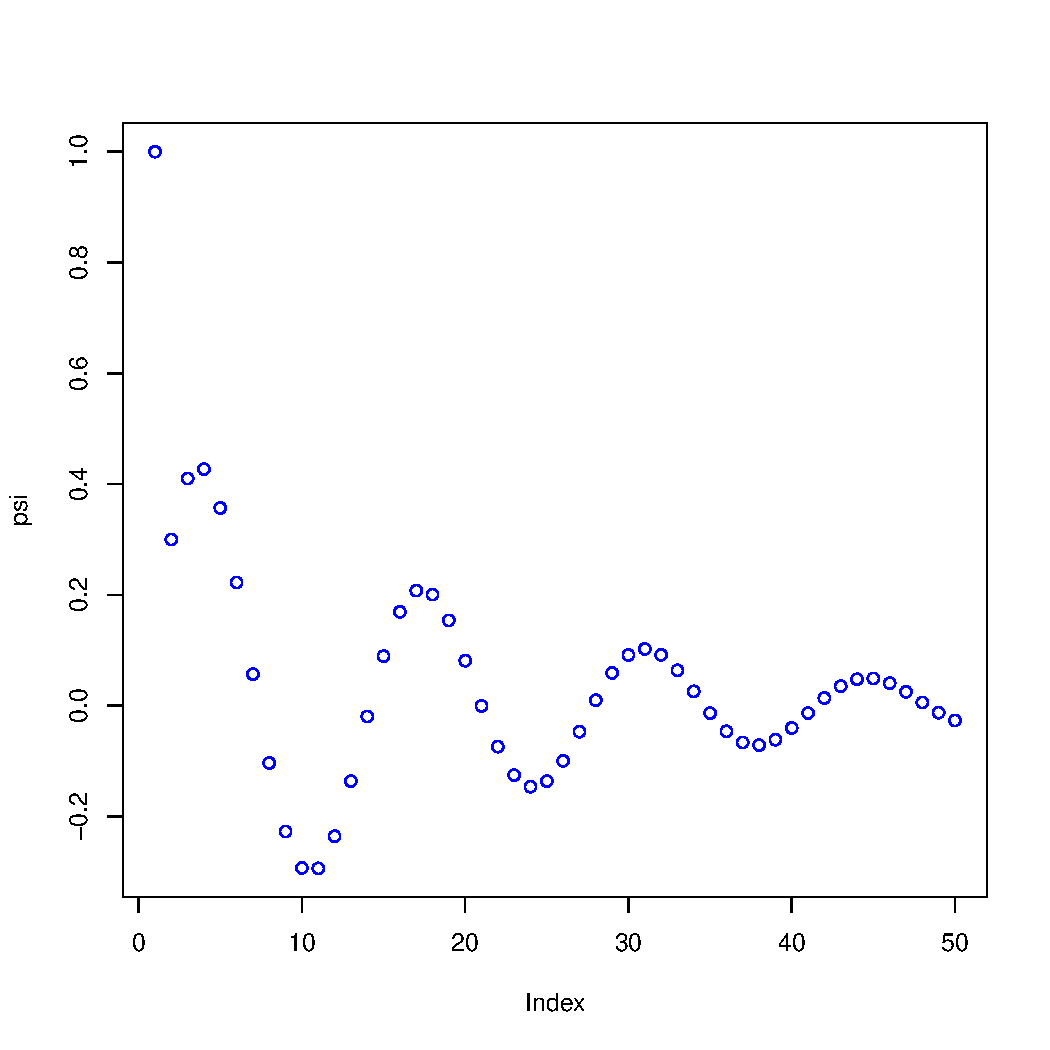
\includegraphics[width=4in]{psi} 
   \caption{Plot of $\psi$ for $j = 0, 50$}
   \label{fig:psi}
\end{figure}

%%%%%%%%%%%%%%%%%%%%%%%%%%%%%%%%%%%%%%%%%%%%%%%%%%%%%%%%%%%%%
%%%%%%%%%%%%%%%%%%%%%%%%%%%%%%%%%%%%%%%%%%%%%%%%%%%%%%%%%%%%%
\section{Problem 4.3}
Consider a causal ARMA(p,q) process. Then
\begin{equation}\label{eq:gamma}
\gamma(h)= \sum_{k=1}^{p}\phi_{k}\gamma(h-k) + \sigma^{2}\sum_{j=0}^{q}\theta_{j+h}\psi_{j}, \quad h\geq 0
\end{equation}

\subsection{Part a: Finding $\{ \gamma(h), h = 0, \cdots, 4\}$ for  ARMA(2,3)}
Expanding (\ref{eq:gamma})  for $p=2, q=3$, we get
\begin{equation}
\begin{aligned}
\gamma(h) &= \sum_{k=1}^{2}\phi_{k}\gamma(h-k) + \sigma^{2}\sum_{j=0}^{3}\theta_{j+h}\psi_{j}\\
&=\phi_{1}\gamma(h-1) + \phi_{2}\gamma(h-2) + \sigma^{2}(\theta_{h}\psi_{0} + \theta_{1+h}\psi_{1} + \theta_{2+h}\psi_{2}+\theta_{3+h}\psi_{3} )
\end{aligned}
\end{equation}
which can also be written as 
\begin{equation}\label{eq:gamma0}
\gamma(h+2) = \phi_{1}\gamma(h+1) + \phi_{2}\gamma(h) + \sigma^{2}(\theta_{h+2}\psi_{0} + \theta_{3+h}\psi_{1} + \theta_{4+h}\psi_{2}+\theta_{5+h}\psi_{3} ).
\end{equation}
From \cite{petter}, page 88, equation (3.2.3) given by
\begin{equation}
\gamma(h) = \sigma^{2}\sum_{j=0}^{\infty}\phi_{j}\psi_{j+|h|}
\end{equation}
holds true for an ARMA(p,q) process. So we can compute $\gamma(0), \gamma(1)$ as 
\begin{equation}
\gamma(0) =  1
\end{equation}

\begin{equation}
\gamma(1) =  \sigma^{2}\sum_{j=0}^{3}\psi_{j}\psi_{j+1}
\end{equation}
And from (\ref{eq:gamma0}) we have 
\begin{equation}
\begin{aligned}
\gamma(0) &= 1\\
\gamma(1) &=  \sigma^{2}\sum_{j=0}^{3}\psi_{j}\psi_{j+1}\\
\gamma(2) &= \phi_{1}\gamma(1) + \phi_{2}\gamma(0) + \sigma^{2}(\theta_{2}\psi_{0} + \theta_{3}\psi_{1} + \theta_{4}\psi_{2}+\theta_{5}\psi_{3} )\\
\gamma(3) &= \phi_{1}\gamma(2) + \phi_{2}\gamma(1) + \sigma^{2}(\theta_{3}\psi_{0} + \theta_{4}\psi_{1} + \theta_{5}\psi_{2}+\theta_{6}\psi_{3} )\\
\gamma(4) &= \phi_{1}\gamma(3) + \phi_{2}\gamma(2) + \sigma^{2}(\theta_{4}\psi_{0} + \theta_{5}\psi_{1} + \theta_{6}\psi_{2}+\theta_{7}\psi_{3} )
\end{aligned}
\end{equation}
or in a matrix equation
\begin{equation}
\left[
 \begin{array}{c}
  \gamma(0) \\ \gamma(1)  \\ \gamma(2)  \\ \gamma(3)  \\ \gamma(4)  
  \end{array}
   \right] = 
   \left[ 
   \begin{array}{c}
    \phi_{1} \\ \phi_{2} 
  \end{array}
  \right]
   \begin{bmatrix}
    0 & 0 \\ 0 & 0 \\ \gamma(1) & \gamma(0) \\ \gamma(2) & \gamma(1) \\ \gamma(3) & \gamma(2)
     \end{bmatrix} 
     +\sigma^{2}
     \left[ 
   \begin{array}{c}
    \sum_{j=0}^{3}\psi_{j}\psi_{j} \\  \sum_{j=0}^{3}\psi_{j}\psi_{j+1} \\\sum_{j=0}^{3}\theta_{j+2}\psi_{j}\\\sum_{j=0}^{3}\theta_{j+3}\psi_{j}\\\sum_{j=0}^{3}\theta_{j+4}\psi_{j}
  \end{array}
  \right]
\end{equation}

%%%%%%%%%%%%%%%%%%%%%%%%%%%%%%%%%%%%%%%%%%%%%%%%%%%%%%%%%%%%%%%%%%
\subsection{Part b: Homogeneous difference equation $\phi(B)\gamma(h)=0$}
From part a) equation (\ref{eq:gamma0}) we had 
\begin{equation}\label{eq:gamma1}
\gamma(h+2) = \phi_{1}\gamma(h+1) + \phi_{2}\gamma(h) + \sigma^{2}(\theta_{h+2}\psi_{0} + \theta_{3+h}\psi_{1} + \theta_{4+h}\psi_{2}+\theta_{5+h}\psi_{3} ).
\end{equation}
For an ARAM(p=2,q=3), for $h\geq 4$, the right hand side of (\ref{eq:gamma1}) is 0, resulting in 
\begin{equation}\label{eq:gamma2}
\gamma(h+2) = \phi_{1}\gamma(h+1) + \phi_{2}\gamma(h) 
\end{equation}
or 
\begin{equation}\label{eq:gamma3}
\gamma(h+2)-\phi_{1}\gamma(h+1)-\phi_{2}\gamma(h)  = 0
\end{equation}

%%%%%%%%%%%%%%%%%%%%%%%%%%%%%%%%%%%%%%%%%%%%%%%%%%%%%%%%%%%%%%%%%%%
\subsection{Part c: Plot of $\{ \gamma(h), h = 0 , \cdots,50  \}$ }
The parameter are given by 
\begin{equation}\label{eq:params1}
\bm{\phi} = (\phi_{1}, \phi_{2}) = (1.7, -0.9), \quad \bm{\theta} = (\theta_{1}, \theta_{2}, \theta_{3}) = (-1.4, 0.8, 0.1) ,\quad \sigma^{2} = 1 .
\end{equation}
and 
\begin{equation}\label{eq:gamma22}
\gamma(h+2) = 1.7\gamma(h+1) -0.9\gamma(h) 
\end{equation}

\clearpage
R code 
\begin{lstlisting}
#initialization for psi
psi0 = 1
psi1 = 0.3
psi2 = 0.41
theta3 = 0.1
psi3 = 1.7*psi2 - 0.9*psi1 + theta3
psi <- c(psi0,psi1,psi2,psi3)
#compute the rest
for (j in 2:48)
  psi[j+2] = 1.7*psi[j+1] - 0.9*psi[j]

#Initialize gamma with gamma0 and gamma1
gamma0 = 0
for (k in 1:5)
  gamma0 = gamma0 + psi[k]*psi[k]

gamma1 = 0
for (k in 1:5)
  gamma1 = gamma1 + psi[k]*psi[k+1]

gamma = c(gamma0,gamma1)
# comute the rest of the gamma's
for (k in 1:48)
  gamma[k+2] = 1.7*gamma[k+1] - 0.9*gamma[k]
print(length(gamma))

#plot
plot(gamma, col='blue')
\end{lstlisting}

We use the R function ARMAacf to comopute $\gamma$ with the following code
\begin{lstlisting}
Rfunction<-ARMAacf( c(1.7,-0.9),c(-1.4,0.8,0.1),50)
plot(Rfunction, col='green')
\end{lstlisting}


\begin{figure}[H] %  figure placement: here, top, bottom, or page
   \centering
   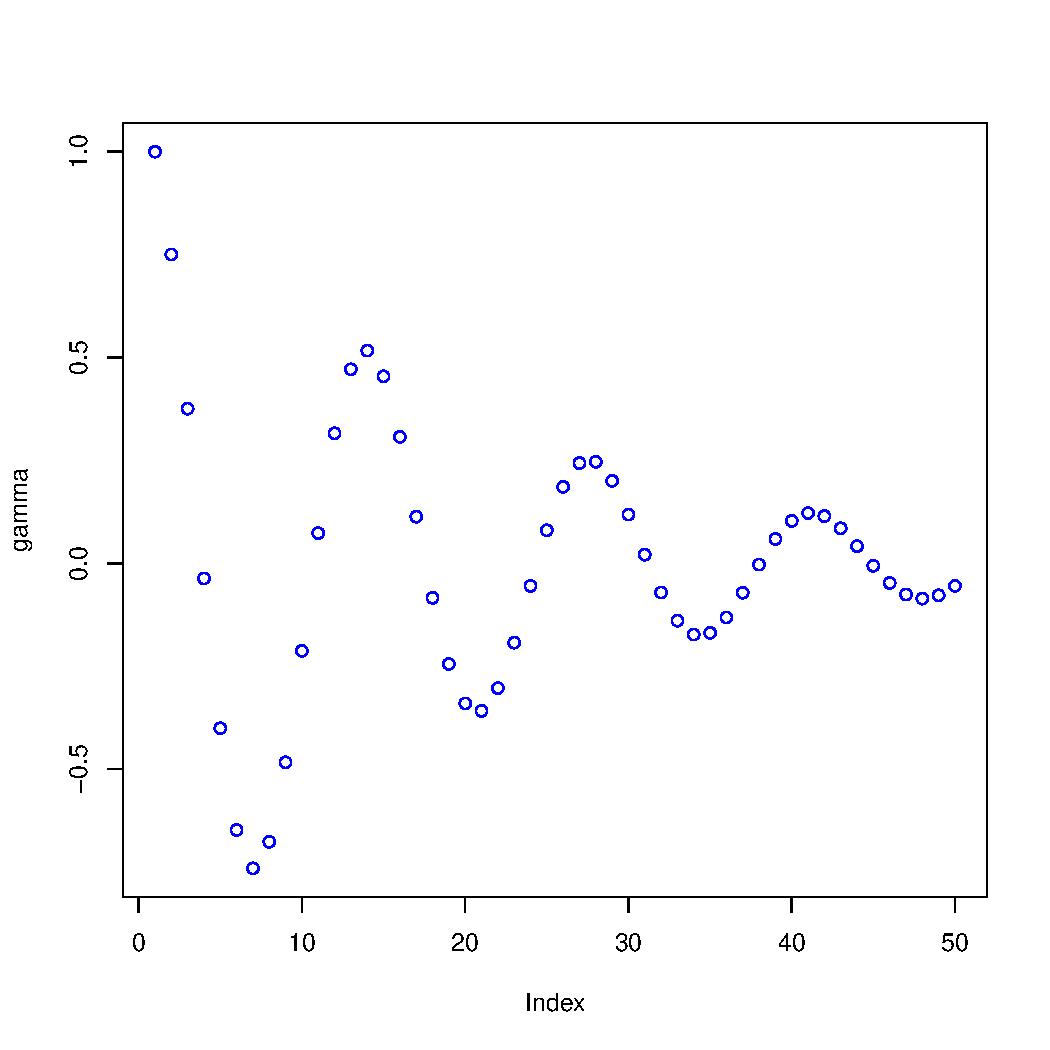
\includegraphics[width=2.5in]{Rplots} 
    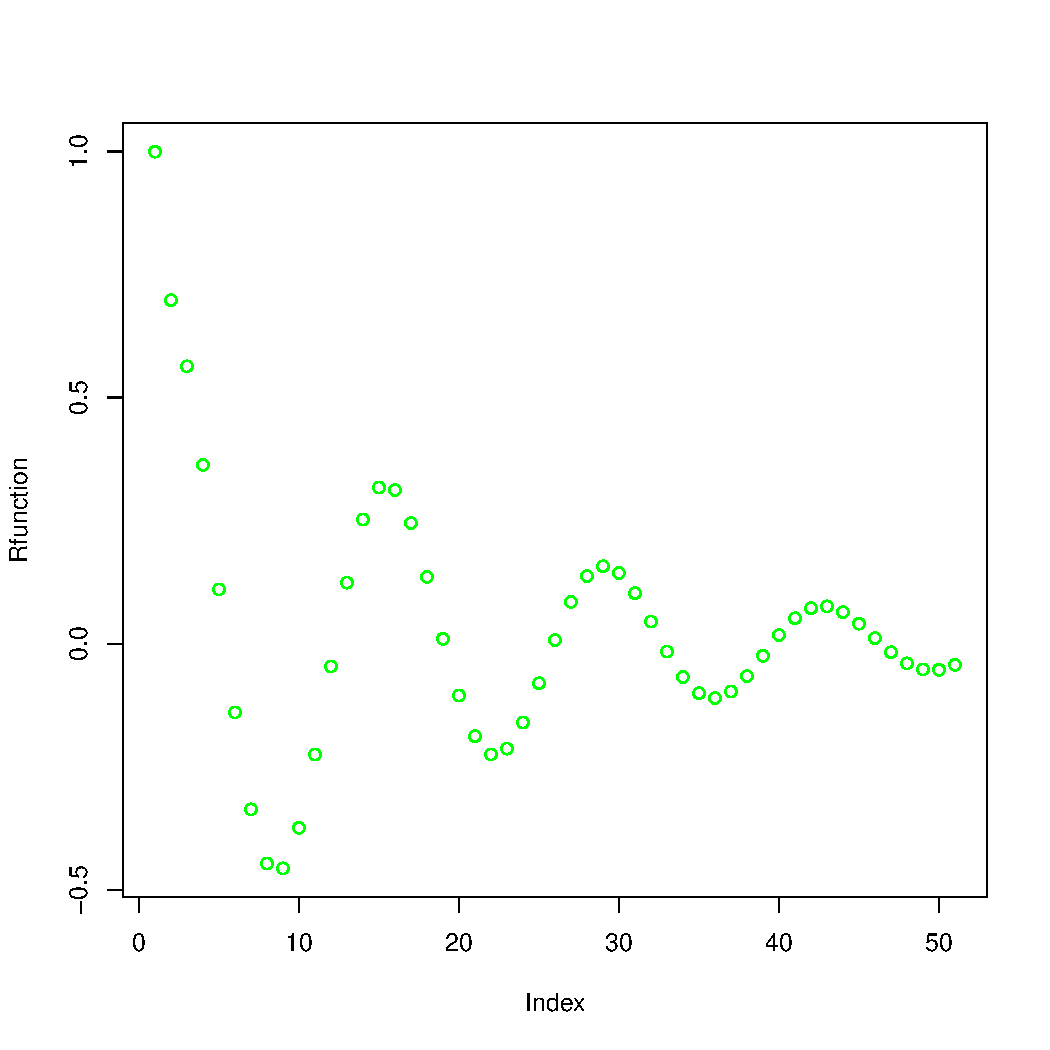
\includegraphics[width=2.5in]{Rfunction} 
   \caption{Plot of $\gamma$ for $j = 0, 50$. Computed in blue vs R function (green)}
   \label{fig:gamma}
\end{figure}
Figure \ref{fig:gamma} shows the computed $\gamma$ versus the $\gamma$ computed with the R function ARMAacf.


%%%%%%%%%%%%%%%%%%%%%%%%%%%%%%%%%%%%%%%%%%%%%%%%%%%%%%%%%%
%%%%%%%%%%%%%%%%%%%%%%%%%%%%%%%%%%%%%%%%%%%%%%%%%%%%%%%%%%
\clearpage
\section{Problem 4.4}
Let $\{X_{t}\}$ be a causal AR(2) process with white noise process $WN(0,\sigma^{2})$,
\begin{equation}\label{eq:main}
X_{t}-\phi_{1}X_{t-1}-\phi_{2}X_{t-2} = Z_{t}, \quad X_{t} = \sum_{j=0}^{\infty}\psi_{j}Z_{t-j}.
\end{equation}

\subsection{Part a: Deduce $\gamma(h) = \sum_{k=1}^{p}\phi_{k}\gamma(h-k)+\delta_{0,h}\sigma^{2}$}
First we know that
\begin{equation}\label{eq:gam}
\gamma(h) = \Cov(X_{t+h}, X_{t}) \Rightarrow \gamma(h-k) = \Cov(X_{t+h}, X_{t-k})
\end{equation}
Multiplying (\ref{eq:main}) by $X_{t+h}$,  and taking the expectation, gives 
\begin{equation}
\begin{aligned}
X_{t+h}X_{t}-\phi_{1}X_{t+h}X_{t-1}-\phi_{2}X_{t+h}X_{t-2} &= X_{t+h}Z_{t}\\
\E[X_{t+h}X_{t}]-\phi_{1}\E[X_{t+h}X_{t-1}]-\phi_{2}\E[X_{t+h}X_{t-2}] &= E[X_{t+h}Z_{t}]\\
\Cov(X_{t+h},X_{t})-\phi_{1}\Cov(X_{t+h},X_{t-1})-\phi_{2}\Cov(X_{t+h},X_{t-2}) &= \Cov(X_{t+h},Z_{t})\\ \nonumber
&= \Cov\left(\sum_{j=0}^{\infty}\psi_{j}Z_{t+h-j},Z_{t}\right)\\
&=\Cov(  \psi_{0}Z_{t+h}+ \psi_{1}Z_{t+h-1}, +\cdots, Z_{t})\\
&=\psi_{0}\Cov(Z_{t+h}, Z_{t}) + \psi_{1}\Cov(Z_{t+h-1}, Z_{t}) + \cdots\\
\Cov(X_{t+h},X_{t})-\phi_{1}\Cov(X_{t+h},X_{t-1})-\phi_{2}\Cov(X_{t+h},X_{t-2}) &= 1\Cov(Z_{t+h},Z_{t}) \\
\gamma(h)- \phi_{1}\gamma(h-1)-\phi_{2}\gamma(h-2) &= \sigma^{2}\delta_{h,0}\\
\gamma(h) - \sum_{k=1}^{p=2}\phi_{k}\gamma(h-k) &= \sigma^{2}\delta_{h,0}\\
\gamma(h) &= \sum_{k=1}^{p=2}\phi_{k}\gamma(h-k) + \sigma^{2}\delta_{h,0}
\end{aligned}
\end{equation}

\subsection{Part b: Some verification}
\begin{equation}
\begin{aligned}
\frac{\gamma(h)}{\gamma(0)} &= \rho(h)\\
&=\phi_{1}\frac{\gamma(h-1)}{\gamma(0)} + \phi_{2}\frac{\gamma(h-2)}{\gamma(0)} + \frac{\sigma^{2}\delta_{h,0}}{\gamma(0)}\\
\end{aligned}
\end{equation}
from which we get
\begin{equation}\label{eq:e1}
\begin{aligned}
\rho(1) &= \phi_{1}\frac{\gamma(0)}{\gamma(0)} + \phi_{2}\frac{\gamma(-1)}{\gamma(0)} + \frac{\sigma^{2}\delta_{1,0}}{\gamma(0)}\\
\rho(1)&=\phi_{1}\frac{\gamma(0)}{\gamma(0)} + \phi_{2}\frac{\gamma(1)}{\gamma(0)} + \frac{\sigma^{2}\delta_{1,0}}{\gamma(0)}\\
\rho(1)&=\phi_{1} + \phi_{2}\rho(1)\\
\rho(1)-\phi_{2}\rho(1)&=\phi_{1} \\
\textcolor{blue}{(1-\phi_{2})\rho(1)} &= \textcolor{blue}{\phi_{1}}
\end{aligned}
\end{equation}
and 

\begin{equation}\label{eq:e2}
\begin{aligned}
\rho(2) &= \phi_{1}\frac{\gamma(1)}{\gamma(0)} + \phi_{2}\frac{\gamma(0)}{\gamma(0)} + \frac{\sigma^{2}\delta_{2,0}}{\gamma(0)}\\
\rho(2)&= \phi_{1}\rho(1) + \phi_{2}\\
\textcolor{blue}{\rho(2) -\phi_{1}\rho(1)} &= \textcolor{blue}{\phi_{2}}\\
\end{aligned}
\end{equation}
and
\begin{equation}\label{eq:e3}
\begin{aligned}
\rho(0) &= \phi_{1}\frac{\gamma(-1)}{\gamma(0)} + \phi_{2}\frac{\gamma(-2)}{\gamma(0)} + \frac{\sigma^{2}\delta_{0,0}}{\gamma(0)}\\
1 &= \phi_{1}\frac{\gamma(1)}{\gamma(0)} + \phi_{2}\frac{\gamma(2)}{\gamma(0)} + \frac{\sigma^{2}}{\gamma(0)}\\
1 &= \phi_{1}\rho(1) + \phi_{2}\rho(2) + \frac{\sigma^{2}}{\gamma(0)}\\
1 -\phi_{1}\rho(1) - \phi_{2}\rho(2) &= \frac{\sigma^{2}}{\gamma(0)}\\
\textcolor{blue}{\gamma(0)(1 -\phi_{1}\rho(1) - \phi_{2}\rho(2))} &= \textcolor{blue}{\sigma^{2}}\\
\end{aligned}
\end{equation}

\subsection{Part c: Solution of equations}
From equation (\ref{eq:e1})
\begin{equation}
(1-\phi_{2})\rho(1) = \phi_{1} \Longrightarrow \rho(1) = \frac{\phi_{1}}{1-\phi_{2}}.
\end{equation}
From equation (\ref{eq:e2})
\begin{equation}
\begin{aligned}
\rho(2) -\phi_{1}\rho(1) &= \phi_{2}\\
\rho(2) -\phi_{1} \frac{\phi_{1}}{1-\phi_{2}} &= \phi_{2}\\
\rho(2) - \frac{\phi^{2}_{1}}{1-\phi_{2}} &= \phi_{2} \Longrightarrow \rho(2) = \phi_{2}+\frac{\phi^{2}_{1}}{1-\phi_{2}},
\end{aligned}
\end{equation}
now inserting the expression of $\rho(1), \rho(2)$ into equation (\ref{eq:e3}) and solving for $\gamma(0)$ we get
\begin{equation}\label{eq:gma}
\begin{aligned}
\gamma(0) &= \frac{\sigma^{2}}{ 1-\phi_{1}\rho(1)-\phi_{2}\rho(2)}\\
\gamma(0)&= \frac{\sigma^{2}}{   1-\phi_{1}\frac{\phi_{1}}{1-\phi_{2}}-\phi_{2}\left( \phi_{2}+\frac{\phi^{2}_{1}}{1-\phi_{2}}\right)   }\\
\end{aligned}
\end{equation}

\subsection{Part d: Boundary condition for causal AR(2) model}
From equation (\ref{eq:gma}), at the boundary we have for a causal model
\begin{equation}
\begin{aligned}
1-\phi_{1}\frac{\phi_{1}}{1-\phi_{2}}-\phi_{2}\left( \phi_{2}+\frac{\phi^{2}_{1}}{1-\phi_{2}}\right) &= 0\\
1-\phi^{2}_{2} - \frac{\phi^{2}_{1}}{1-\phi_{2}} -\frac{  \phi_{2}\phi^{2}_{1}   }{1-\phi_{2}} &= 0\\
(1-\phi^{2}_{2})(1-\phi_{2} ) -\phi^{2}_{1} - \phi_{2}\phi^{2}_{1} &= 0\\
(1+\phi_{2})(1-\phi_{2})(1-\phi_{2}) &= \phi^{2}_{1}(1+\phi_{2})\\
(1-\phi_{2})(1-\phi_{2}) &= \phi^{2}_{1}\\
(1-\phi_{2})^{2} &= \phi^{2}_{1}\\
(1-\phi_{2})^{2}-\phi^{2}_{1} &=0\\
(1-\phi_{2}+\phi_{1})(1-\phi_{2}-\phi_{1})& = 0
\end{aligned}
\end{equation}
From which we get 
\begin{equation}
1-\phi_{2}+\phi_{1} = 0 \Longrightarrow \phi_{2}-\phi_{1} = 1
\end{equation}

\begin{equation}
1-\phi_{2}-\phi_{1}  = 0 \Longrightarrow \phi_{2}+\phi_{1} = 1
\end{equation}
and solving for $\phi_{2}$ we get
\begin{equation}
\phi_{2} = 1
\end{equation}
And we have 
\begin{equation}
\begin{aligned}
\phi_{2}& = 1\\
\phi_{2}-\phi_{1} &= 1\\
\phi_{2}+\phi_{1} &= 1
\end{aligned}
\end{equation}

\subsection{Part e: Finding $\E[X_{3}|X_{1}]$}
\begin{equation}
\begin{aligned}
\E[X_{3}|X_{1}] &=\E\left[\sum_{j=0}^{\infty}\psi_{j}Z_{3-j}\bigg|\sum_{j=0}^{\infty}\psi_{j}Z_{1-j}\right] \\
&=\E\left[ \psi_{0}Z_{3}+\psi_{1}Z_{2}+\cdots \bigg| \sum_{j=0}^{\infty}\psi_{j}Z_{1-j}    \right]\\
&=\psi_{0}\E\left[ Z_{3}\bigg|\sum_{j=0}^{\infty}\psi_{j}Z_{1-j}    \right] + \psi_{1}\E\left[ Z_{2}\bigg|\sum_{j=0}^{\infty}\psi_{j}Z_{1-j}    \right] +\cdots\\
&=\psi_{0}\E\left[  Z_{3}|\psi_{0}Z_{1}+\psi_{1}Z_{0}+\cdots  \right]+\psi_{1}\E\left[  Z_{2}|\psi_{0}Z_{1}+\psi_{1}Z_{0}+\cdots  \right]+\cdots\\
&=\psi_{0}\left(   \psi_{0}\E[Z_{3}|Z_{1}]+\psi_{1}\E[Z_{3}|Z_{0}]+\cdots  \right) +  \psi_{1}\left(   \psi_{0}\E[Z_{2}|Z_{1}]+\psi_{1}\E[Z_{2}|Z_{0}]+\cdots  \right) + \cdots\\
&=\psi_{0}\sum_{j=0}^{\infty}\psi_{j}\E[Z_{3}|Z_{1-j}] + \psi_{1}\sum_{j=0}^{\infty}\psi_{j}\E[Z_{2}|Z_{1-j}] +\cdots\\
&=\sum_{k=0}^{\infty}\psi_{k}\left(\sum_{j=0}^{\infty}\psi_{j}\E[Z_{3-k}|Z_{1-j}]\right)
\end{aligned}
\end{equation}

\subsection{Part f: Asymptotic covariance matrix}
setting
\begin{equation}
\Gamma_{p} = \{ \gamma(i-j), 1\leq i,j \leq p  \}
\end{equation}
We compute $\sigma^{2}\Gamma_{1}^{-1}$ and $\sigma^{2}\Gamma_{2}^{-1}$ as follow:

\begin{equation}
   \sigma^{2}\Gamma_{1}=
  \sigma^{2} \left[ {\begin{array}{cc}
   \gamma(0)  \\
  \end{array} } \right]
\end{equation}

\begin{equation}
   \sigma^{2}\Gamma_{2}=
  \sigma^{2} \left[ {\begin{array}{cc}
   \gamma(0) & \gamma(1) \\
   \gamma(1)& \gamma(0) \\
  \end{array} } \right]
\end{equation}
and 
\begin{equation}
   \sigma^{2}\Gamma_{1}^{-1}=
  \sigma^{2} \left[ {\begin{array}{cc}
   \frac{1}{\gamma(0)}  \\
  \end{array} } \right]
\end{equation}

\begin{equation}
   \sigma^{2}\Gamma_{2}^{-1}=
\frac{\sigma^{2}}{\gamma(0)^{2}-\gamma(1)^{2}} \left[ {\begin{array}{cc}
   \gamma(0) & -\gamma(1) \\
   -\gamma(1)& \gamma(0) \\
  \end{array} } \right]
\end{equation}
Where 
\begin{equation}
\gamma(h) = \sigma^{2}\delta_{h,0} 
\end{equation}
so that
\begin{equation}
   \sigma^{2}\Gamma_{1}^{-1}=
  \sigma^{2} \left[ {\begin{array}{cc}
   \frac{1}{\sigma^{2}}  \\
  \end{array} } \right]
  = 
  \sigma^{2} \left[ {\begin{array}{cc}
   1  \\
  \end{array} } \right]
\end{equation}

\begin{equation}
   \sigma^{2}\Gamma_{2}^{-1}=
\sigma^{2} \left[ {\begin{array}{cc}
   1 & 0 \\
   0& 1 \\
  \end{array} } \right]
\end{equation}


%\begin{lstlisting}
%\end{lstlisting}



\begin{thebibliography}{9}
\bibitem{petter} 
Petter J. Brockwell. Richard A. Davis
\textit{Introduction to Time Series and Forecasting}. 
Springer. Second edition. 2001
 
\end{thebibliography}


\end{document}  